\documentclass[12pt]{article}

\usepackage[ngerman]{babel}
\usepackage[utf8]{inputenc}
\usepackage[scale=0.80]{geometry}
\usepackage{amsmath}
\usepackage{amssymb}
\usepackage{graphicx}
\usepackage{fancyhdr}
\usepackage{gensymb}

\renewcommand{\familydefault}{\sfdefault}
\renewcommand{\arraystretch}{1.25}
\setlength{\headheight}{28pt}
\pagestyle{fancy}

\lhead{\textbf{Datenbanksysteme II}\\
\textbf{Lösung von Aufgabe 4}}
\rhead{\textbf{Felix Wolff, Markus Petrykowski}\\
\textbf{Übungsgruppe B}}
\renewcommand{\footrulewidth}{0pt}

\begin{document}

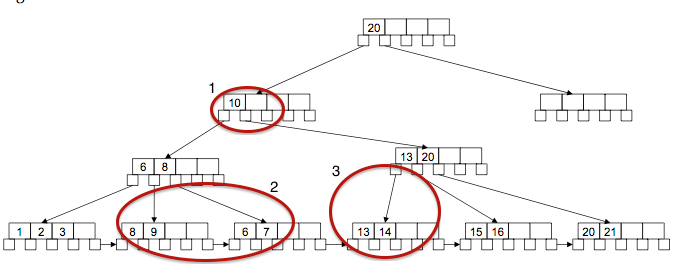
\includegraphics[width=\textwidth]{B+Baum_falsch.png}

\begin{enumerate}
    \item In jedem Knoten müssen mindestens 3 Elemente vorhanden sein

    \item In diesem Fall müssten die beiden Zeiger einfach vertauscht werden um
        den Fehler zu korrigieren. Denn Der Pointer der rechts von einem Element
        ist zeigt auf einen Knoten, der nur Elemente enthält die größer als das
        'Vaterelement' sind. Für die linke Seite gilt es Analog mit dem
        Unterschied das der linke Pointer auf kleinere Werte zeigt

    \item Hier ist ein ähnlicher Fehler wie bei Punkt 2. Der linke Pointer des
        Elements '13' zeigt auf Elemente die größer bzw. gleich dem
        'Vaterelement' sind. Um den Fehler hier zu beheben, könnte man z.B. die
        13 durch eine 15 ersetzen.

    \item Der leere rechte Block, auf den der rechte Zeiger der Wurzel zeigt,
        wird als nicht weiter beschriebener Teilbaum verstanden. Ansonsten ist
        er selbstverständlich auch ein Fehler.
 
\end{enumerate}

\end{document}
% vim: tw=80
